\section{java.util.Map}

\frame{\frametitle{java.util.Map}
\begin{center}
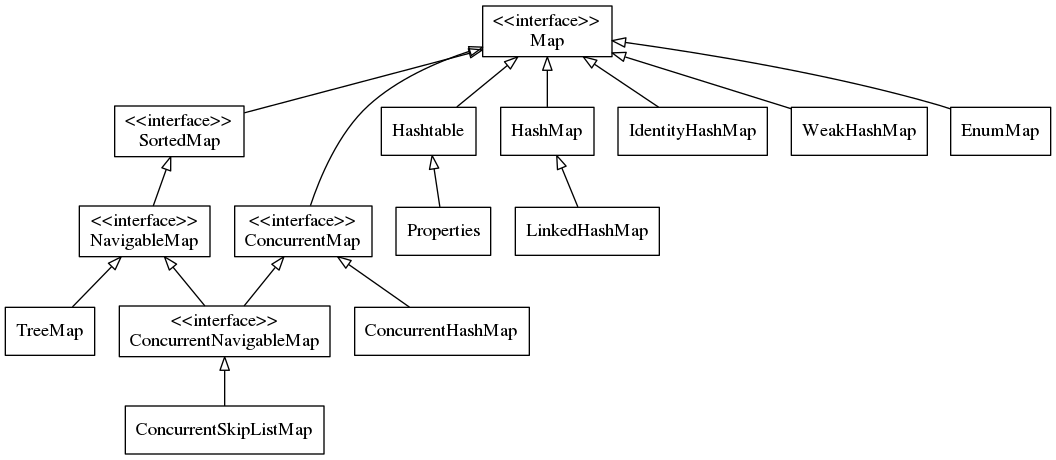
\includegraphics[width=0.9\textwidth]{java.util.Map/java_util_Map_overview}
\end{center}
}

%%%%%%%%%%%%%%%%%
%    HashMap    %
%%%%%%%%%%%%%%%%%

\frame{
\frametitle{HashMap}
\begin{center}
  \begin{itemize}[<+->]
    \item seit 1.2
    \item null keys und values erlaubt
    \item wie Hashtable, aber mit nulls und nicht thread-safe
    \item get/put in \O{1}
    \item nicht thread-safe
    \item fail-fast iterator
  \end{itemize}
\end{center}
}

\begin{frame}[fragile]
\frametitle{HashMap - interne Struktur}
\begin{itemize}[<+->]
  \item capacity = Anzahl an buckets, initialCapacity = Start capacity
  \item loadFactor = Ab wann automatisch rehash
  \item rehash: interne Datenstruktur wird neu gebaut $\Rightarrow$ Kapazität steigt um Faktor 2
  \item Konstruktor: initialCapacity und loadFactor \\
	\verb+DEFAULT_LOAD_FACTOR = 0.75f+ \\
	\verb+DEFAULT_INITIAL_CAPACITY = 1 << 4; // = 16+
  \item wenn $number\ entries \geq loadFactor * capacity$ dann rehash
  \item wenn viele puts, dann sollte initialCapacity groß genug sein, um Anzahl an rehashes klein zu halten
\end{itemize}
\end{frame}

\frame{
\frametitle{HashMap - Zugriffszeiten}
\begin{center}
  \begin{tabular}{l|l}
  Operation        & Laufzeit \\\hline
  get              & \O{1} \\
  put              & \O{1} \\
  \end{tabular}
\end{center}
}

\frame{
\frametitle{HashMap - Wann nehmen?}
\begin{center}
  Synchronisation egal, \\\pause
  Ordnung egal, \\\pause
  oft get/put
\end{center}
}


%%%%%%%%%%%%%%%%%
% LinkedHashMap %
%%%%%%%%%%%%%%%%%


\frame{
\frametitle{LinkedHashMap}
\begin{center}
  \begin{itemize}[<+->]
    \item null erlaubt
    \item add, contains, remove \O{1}
    \item iteration = \O{size}, HashMap = \O{capacity}, schneller falls $size < capacity$
    \item initial capacity and load factor wie HashMap
    \item not synchronized, nicht thread-safe
    \item fail-fast iterator
    \item Reihenfolge nach Einfügen (insertion-order)
  \end{itemize}
\end{center}
}

\begin{frame}[fragile]
\frametitle{LinkedHashMap - LRU-Cache}
  \begin{block}{Least Recently Used}
    \begin{enumerate}[<+->]
      \item \textit{new LinkedHashMap(initialCapacity, loadFactor, accessOrder)} \\
	    accessOrder = true für access-order, von least nach most-recently \\
      \item um nach put / putAll zu aktualisieren removeEldestEntry überschreiben
	  \begin{lstlisting}
     @Override
     protected boolean removeEldestEntry(Map.Entry eldest) {
        return size() > 100;
     }
	  \end{lstlisting}
    \end{enumerate}
  \end{block}
\end{frame}

\frame{\frametitle{LinkedHashMap - Zugriffszeiten}
\begin{center}
  \begin{tabular}{l|l}
  Operation        & Laufzeit \\\hline
  add              & \O{1} \\
  contains         & \O{1} \\
  remove           & \O{1} \\
  get              & \O{TODO} \\
  put              & \O{TODO} \\
  \end{tabular}
\end{center}
}

\frame{\frametitle{LinkedHashMap - Wann nehmen?}
\begin{center}
  Reihenfolge wichtig oder \\\pause
  schnelle Iteration (schneller als HashMap)
\end{center}
}


%%%%%%%%%%%%%%%%%%%%
% IdentityHashMap  %
%%%%%%%%%%%%%%%%%%%%

\frame{
\frametitle{IdentityHashMap}
\begin{center}
  \begin{itemize}[<+->]
    \item hashed mit System.identityHashCode(Object) anstatt der hashCode Implementierung
    \item Referenz-Gleichheit anstatt equals \\
	  \textit{if (k1==k2)} anstatt \\
	  \textit{if (k1==null ? k2==null : k1.equals(k2))} (HashMap)
    \item betrifft nur keys
    \item verletzt bewusst den Map-Vertrag ''equals() zum Vergleichen''
    \item null keys/values erlaubt
    \item keine Reihenfolge
    \item get/put in O(1)
    \item expected maximum size sollte genutzt werden, erweitern ist teuer
    \item nicht thread-safe
    \item fail-fast iterator
  \end{itemize}
\end{center}
}

\frame{
\frametitle{IdentityHashMap - Wann nehmen?}
\begin{center}
  nur wenn Referenz-Gleichheit gebraucht wird
\end{center}
}


%%%%%%%%%%%%%%%%%%%%
%   WeakHashMap    %
%%%%%%%%%%%%%%%%%%%%

\frame{
\frametitle{WeakHashMap}
\begin{center}
  \begin{itemize}[<+->]
    \item weak keys (als weak reference)
    \item GC räumt Key weg auch wenn es einen Value gibt
    \item Wenn ein Key weggeräumt wurde, wird der Value (hard reference) aus der Map entfernt
    \item[$\Rightarrow$] values sollten nicht (in)direkt auf ihre keys verweisen, sonst werden sie nicht GC't
    \item[$\Rightarrow$] workaround: values in WeakReference einpacken
    \item null key, null value supported
    \item Effizienz wie HashMap
    \item nicht thread-safe
    \item fail-fast iterator
  \end{itemize}
\end{center}
}

\frame{\frametitle{WeakHashMap - Wann nehmen?}
\begin{center}
  object reference als key und GC soll die Map beaufsichtigen (also sehr selten) \\\pause
  data cache implementations \\\pause
  EIGENTLICH \textbf{nie}: wenn cache, dann guava oder javax.cache (JSR107) oder ...
\end{center}
}


%%%%%%%%%%%%%%%%%%%%%
% ConcurrentHashMap %
%%%%%%%%%%%%%%%%%%%%%

\frame{
\frametitle{ConcurrentHashMap}
\begin{center}
  \begin{itemize}[<+->]
    \item ist keine spezielle HashMap, wie LinkedHashMap
    \item ist wie Hashtable (bspw. thread-safe)
    \item lesende Operationen blockieren nicht
    \item jeglichen Zugriff blockieren ist nicht möglich
    \item kann Hashtable komplett ersetzen, falls man nur auf thread-safety angewiesen ist, nicht auf die Synchronisations-Details von Hashtable
    \item read-Methoden stellen (irgend)einen Zustand dar, vielleicht auch nur die Hälfte von einem putAll
    \item fail-safe iterator
    \item Änderung der Größe ist teuer
    \item Größe optimieren: Konstruktor-Parameter concurrencyLevel gibt Anzahl parallel schreibender Threads an
    \item kein null erlaubt (weder key noch value)
  \end{itemize}
\end{center}
}


\frame{\frametitle{ConcurrentHashMap - Wann nehmen?}
\begin{center}
  wenn eine thread-safe Map benötigt wird oder \\\pause
  Hashtable ersetzt werden soll oder \\\pause
  fail-safe Iterator
\end{center}
}


%%%%%%%%%%%%%%%%%
%   Hashtable   %
%%%%%%%%%%%%%%%%%

\frame{
\frametitle{Hashtable}
\begin{center}
  \begin{itemize}[<+->]
    \item fail-fast iterator
    \item thread-safe
    \item seit 1.0
    \item keine null-keys / values
    \item keys müssen hashCode/equals implementieren
    \item (initial) capacity and load factor: für Speicher- und Laufzeit-Optimierung (bspw. rehash)
    \item alles mit public ist synchronisiert
  \end{itemize}
\end{center}
}

\frame{\frametitle{Hashtable - Wann nehmen?}
\begin{center}
  \textbf{Gar nicht mehr} \\\pause
  Wenn thread-safe nicht nötig, dann \textbf{HashMap} \\
  Wenn thread-safe nötig, dann \textbf{ConcurrentHashMap}
\end{center}
}


%%%%%%%%%%%%%%%%%
%   Properties  %
%%%%%%%%%%%%%%%%%

\frame{\frametitle{Properties}
\begin{center}
  \begin{itemize}[<+->]
    \item seit 1.0
    \item extends Hashtable\textless\,Object,Object\textgreater
    \item setProperty(String key, String value) nutzen anstatt put/putAll (lassen Object zu)
    \item Konstruktor nimmt eine Properties Instanz als default-Werte
    \item load(Reader) / store(Writer, String)
    \item store schreibt keine defaults
    \item Kommentare mit \# sind konfigurierbar unterstützt
    \item Leerzeichen in keys und führende in values werden mit ''\textbackslash\ '' geschrieben
    \item thread-safe, weil Hashtable
    \item obwohl von Hashtable abgeraten wird, wird von Properties (noch) nicht abgeraten
  \end{itemize}
\end{center}
}

\frame{\frametitle{Properties - Meine Meinung}
  \begin{block}{falsch implementiert}
    extends Hashtable\textless\,Object,Object\textgreater , man soll aber nur mit Strings arbeiten $\Rightarrow$ wieso dann nicht extends Hashtable\textless\,String,String\textgreater ?
  \end{block}
}

\frame{\frametitle{Properties - Wann nehmen?}
\begin{center}
  key-value-Paare als Konfiguration, die man persistieren möchte (siehe load/store) \\\pause
  Alternative: java.util.prefs.Preferences
\end{center}
}


%%%%%%%%%%%%%%%%%%%%
%      EnumMap     %
%%%%%%%%%%%%%%%%%%%%

\frame{
\frametitle{EnumMap}
\begin{center}
  \begin{itemize}[<+->]
    \item keys = enum values
    \item intern ein Array pro enum-value
    \item sehr kompakt und effizient
    \item Reihenfolge ist die, wie die Enums deklariert sind
    \item weakly consistent iterators
    \item keine null keys, aber null values erlaubt
    \item nicht thread-safe
    \item basic operations in \O{1}
  \end{itemize}
\end{center}
}

\frame{\frametitle{EnumMap - Wann nehmen?}
\begin{center}
  wenn keys enums sind
\end{center}
}


%%%%%%%%%%%%%%%%%
%    TreeMap    %
%%%%%%%%%%%%%%%%%

\frame{
\frametitle{TreeMap}
\begin{center}
  \begin{itemize}[<+->]
    \item fail-fast iterator
    \item nicht thread-safe
    \item nutzt compareTo anstatt equals/hashcode
    \item intern Red-Black-Tree
    \item Reihenfolge: Natürliche Ordnung oder Comparator
    \item containsKey, get, put and remove in \O{log(n)}
    \item equals und compareTo müssen konsistent sein \\
	  $equals \Leftrightarrow compareTo == 0$
    \item Map.Entry Paar (von firstEntry, lastEntry, ...) ist Snapshot, Entry.setValue ist nicht möglich
  \end{itemize}
\end{center}
}

\frame{\frametitle{TreeMap - Zugriffszeiten}
\begin{center}
  \begin{tabular}{l|l}
  Operation        & Laufzeit  \\ \hline
  add              & \O{TODO}  \\
  contains         & \O{TODO}  \\
  containsKey      & \O{log(n)} \\
  remove           & \O{log(n)} \\
  get              & \O{log(n)} \\
  put              & \O{log(n)} \\
  \end{tabular}
\end{center}
}

\frame{\frametitle{TreeMap - Wann nehmen?}
\begin{center}
  wenn man eine sortierte / navigierbare Map braucht, die nicht thread-safe ist
\end{center}
}


%%%%%%%%%%%%%%%%%%%%%%%%%
% ConcurrentSkipListMap %
%%%%%%%%%%%%%%%%%%%%%%%%%

\frame{
\frametitle{ConcurrentSkipListMap}
\begin{center}
  \begin{itemize}[<+->]
    \item Reihenfolge: Natürliche Ordnung oder Comparator
    \item concurrent variant von SkipLists \href{https://en.wikipedia.org/wiki/Skip_list}{Wikipedia SkipList} \\
    \item[] entspricht in etwa einer binären Suche bei der Suche können Elemente aufgrund Verlinkung übersprungen werden (skip)
    \item[] einfügen, suchen, löschen in \O{log(n)}
    \item thread-safe
    \item weakly consistent iterators
    \item aufsteigende Iteration ist schneller als absteigende
    \item Map.Entry Methoden unterstützen kein Entry.setValue (auch entrySet nicht)
    \item size-Methode ist nicht in konstanter Zeit: Iteration über alle Element und ein valid-Check
    \item putAll, equals, toArray, containsValue, und clear sind nicht zwingend atomar
    \item weder null key noch null value
  \end{itemize}
\end{center}
}

\frame{\frametitle{ConcurrentSkipListMap - Wann nehmen?}
\begin{center}
  wenn man eine sortierte / navigierbare Map braucht, die thread-safe ist und man keine null-Keys/Values hat
\end{center}
}


%%%%%%%%%%%%%%%%%%%%%%%%%
%       Übersicht       %
%%%%%%%%%%%%%%%%%%%%%%%%%

\frame{\frametitle{Map - Übersicht}
\begin{center}
  \resizebox{\textwidth}{!}{
    \begin{tabular}{l|c|c|c|c}
			    & thread-safe &  Iterator &    Reihenfolge       &         nulls          \\ \hline
      HashMap               &     nein    & fail-fast &                      &        erlaubt         \\
      LinkedHashMap         &     nein    & fail-fast & insertion / access   &        erlaubt         \\
      IdentityHashMap       &     nein    & fail-fast &                      &        erlaubt         \\
      WeakHashMap           &     nein    & fail-fast &                      &        erlaubt         \\
      ConcurrentHashMap     &      ja     & fail-safe &                      & weder key noch value   \\
      Hashtable             &      ja     & fail-fast &                      & weder key noch value   \\
      Properties            &      ja     & fail-fast &                      & weder key noch value   \\
      EnumMap               &     nein    &   weakly  &     Enum-Order       &        values          \\
      TreeMap               &     nein    & fail-fast & natural / Comparator & values oder Comparator \\
      ConcurrentSkipListMap &      ja     &   weakly  & natural / Comparator & weder key noch value   \\
    \end{tabular}
  }
\end{center}
}
